% Autor: Alfredo Sánchez Alberca (email:asalber@ceu.es)
\begin{tikzpicture}[every label/.style={text=color1}]
\tikzstyle{node} = [align=center, node distance=1cm]; 
\tikzstyle{arrow} = [-latex, color1, line width=10pt];

\node (population) [label=90:Población] at (0,5) {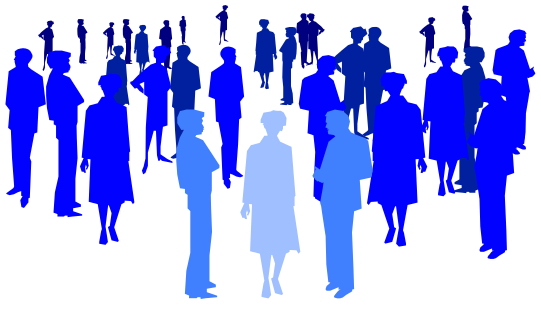
\includegraphics[height=2cm]{img/introduccion/poblacion.pdf}}; 
\node (sample) [label=-90:Muestra] at (0,0) {\includegraphics[height=2cm]{img/introduccion/muestra.png}};
\node at (-0.5,2.6) [fill=color1,single arrow,shape border rotate=270,text=white, minimum width=1.2cm]{
\rotatebox{90}{Deducción}\phantom{}};
\node[node] at (-2,2.5) {De lo general\\ a lo particular};
\pause
\node at (0.5,2.4) [fill=color1,single arrow,shape border rotate=90,text=white, minimum width=1.2cm]{
\rotatebox{-90}{Inducción}\phantom{}};
\node[node] at (2.1,2.5) {De lo particular\\ a lo general};
\end{tikzpicture} 